\documentclass[a4paper, 12pt]{article}
\newcommand{\template}{../../../../Templates}
\usepackage{\template/package}
\graphicspath{{../../../../Assets}}

\newcommand{\Titolo}{Verbale esterno - Imola Informatica}
\newcommand{\Gruppo}{SWEnergy}
\newcommand{\Data}{24/11/2023}
\newcommand{\Mail}{\href{mailto:project.swenergy@gmail.com}{project.swenergy@gmail.com}}
\newcommand{\Versione}{0.1.0}
\newcommand{\Descrizione}{Verbale riguardante la prima chiamata con l'azienda
Imola Informatica dopo l'acquisizione dell'appalto. Sono state poste le domande
in merito all'organizzazione del lavoro e sui casi d'uso.}
\newcommand{\Stato}{Verificato}
\newcommand{\Redattori}{Carlo Rosso}
\newcommand{\Verificatori}{Davide Mafferi}
\newcommand{\ApprovatoriInterni}{}
\newcommand{\ApprovatoriEsterni}{Alessandro Staffolani}

\newcommand{\Titolo}{Valutazione capitolati}
\newcommand{\Gruppo}{SWEnergy}
\newcommand{\Data}{29/10/2023}
\newcommand{\Mail}{\href{mailto:project.swenergy@gmail.com}{project.swenergy@gmail.com}}
\newcommand{\Versione}{0.8.0}
\newcommand{\Descrizione}{
	L'analisi dei capitolati fa riferimento ai documenti presentati al link: \\
	\href{https://www.math.unipd.it/~tullio/IS-1/2023/Progetto/Capitolati.html}{Capitolati 2023}
}
\newcommand{\Stato}{Non approvato}
\newcommand{\Redattori}{
	Alessandro Tigani Sava \\ 
	& Carlo Rosso		\\
	& Davide Maffei		\\
	& Giacomo Gualato	\\
	& Matteo Bando 		\\ 
	& Niccolò Carlesso
}
\newcommand{\Verificatori}{Alessandro Tigani Sava \\ & Nome 2}
\newcommand{\Approvatori}{Nome 1}
\newcommand{\Responsabile}{}

\newcommand{\copertina}{    
	\begin{titlepage}
		\vspace*{-3.5cm}
    	\makebox[\textwidth]{
\includegraphics[width=\paperwidth]{img/header.png}}
		\begin{center}
			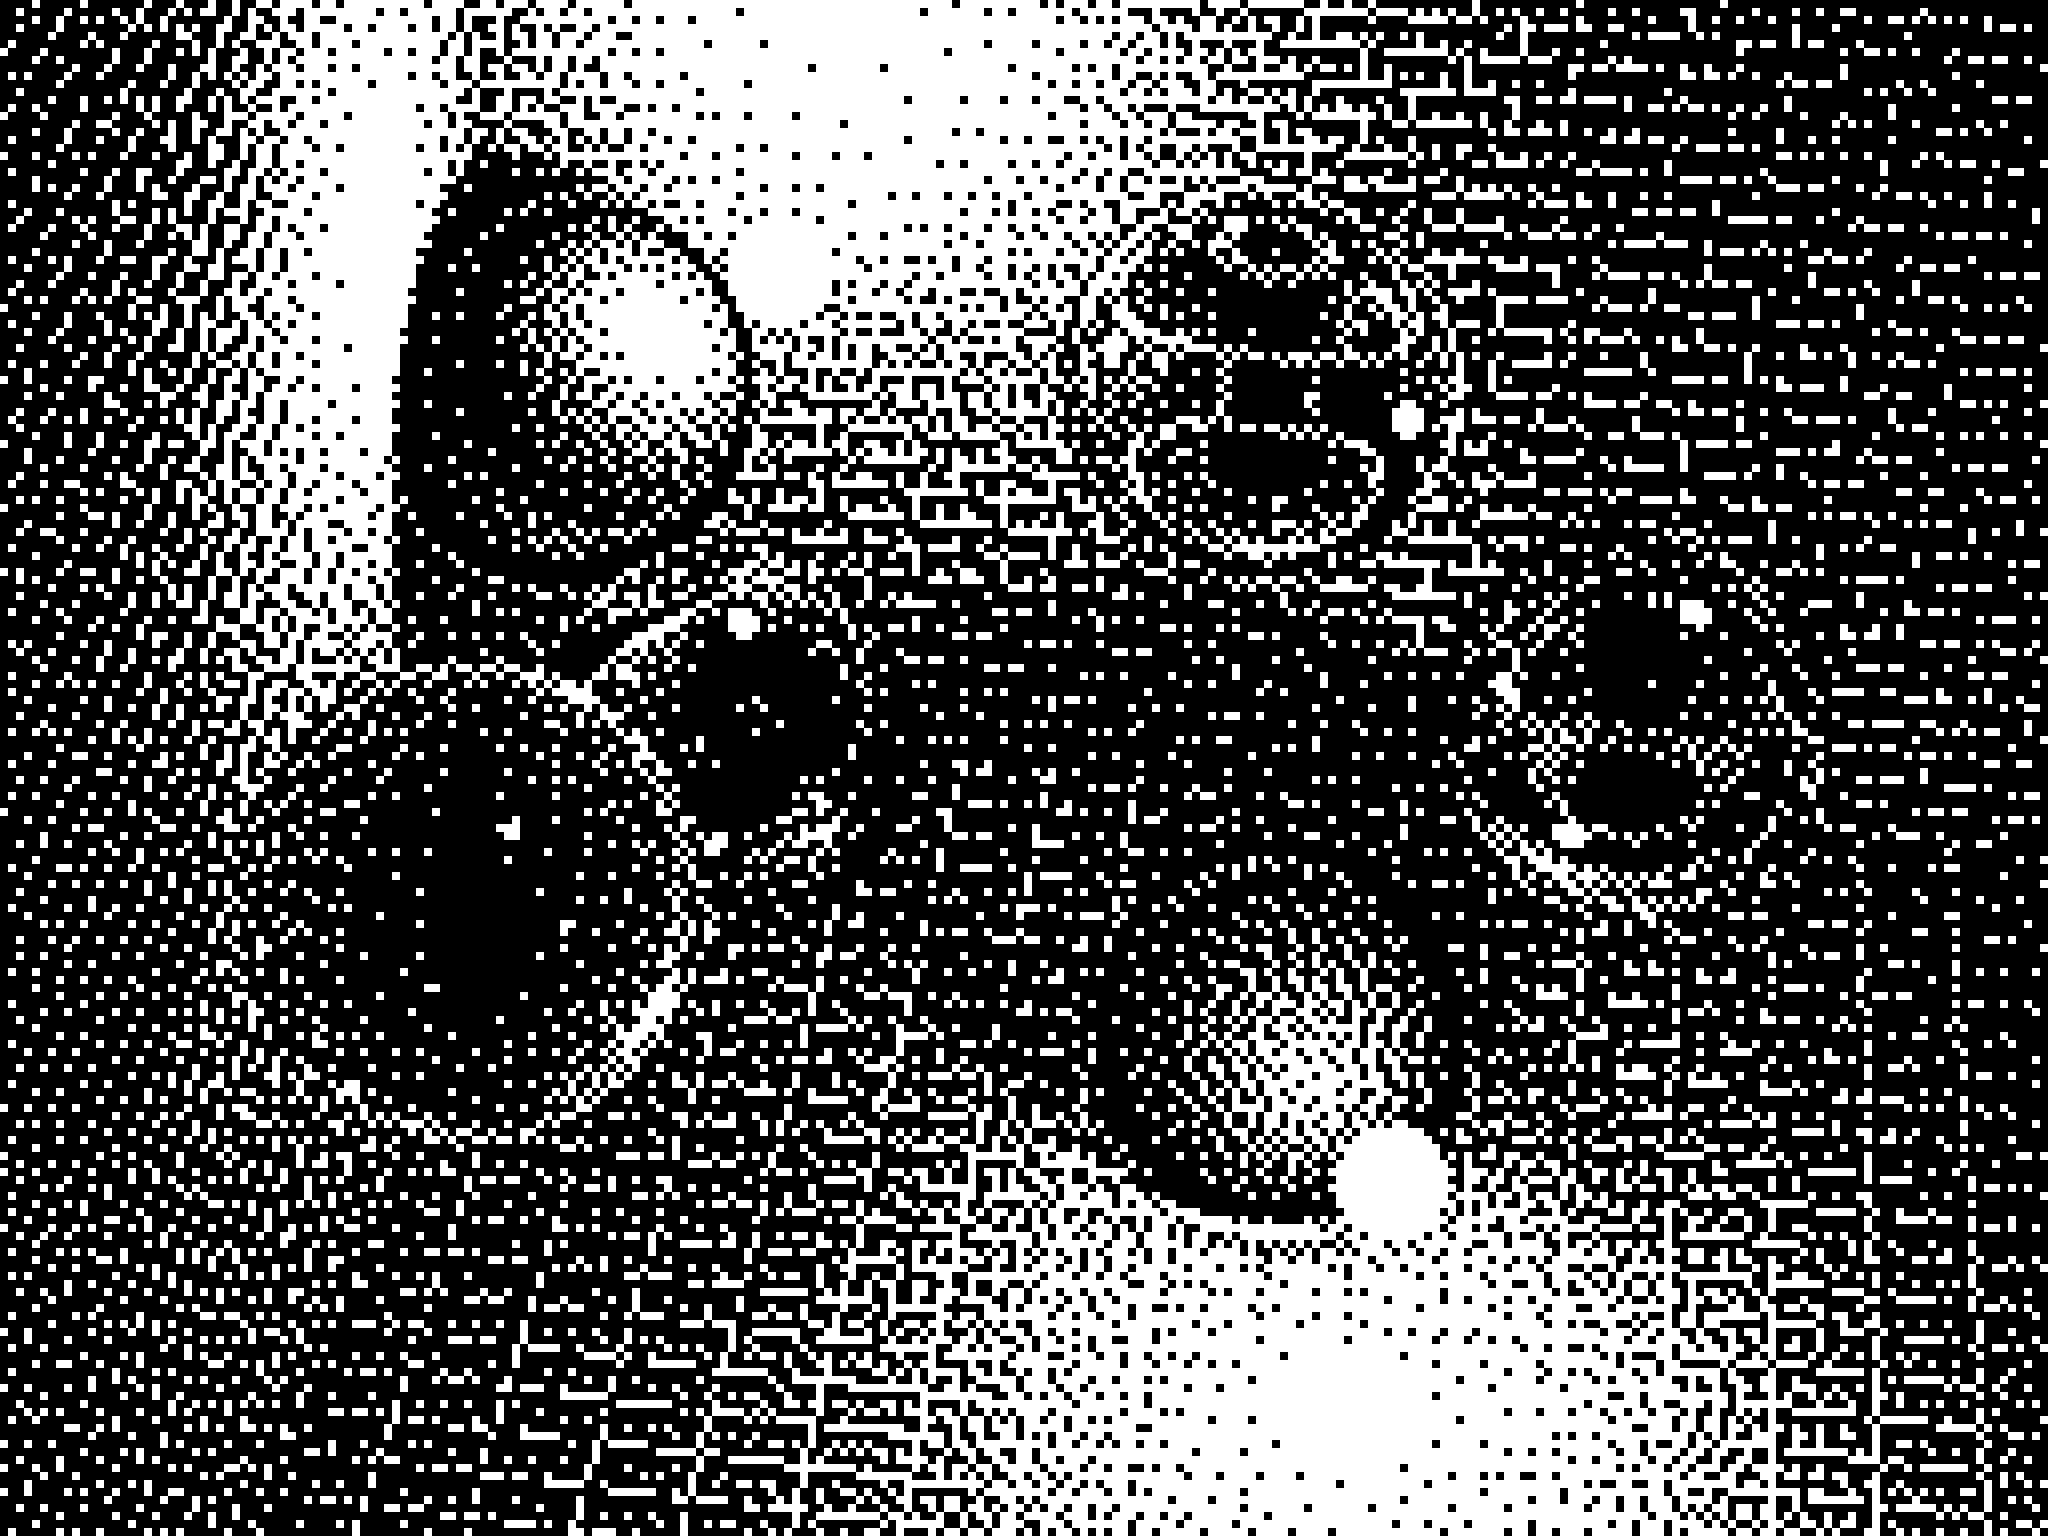
\includegraphics[width=1\textwidth]{img/logo}	\\
			\vspace{1cm}
			\Mail{}	\\
			\vspace{0.5cm}
			\textbf{\begin{LARGE} \Titolo \end{LARGE}}	\\
			\vspace{1cm}
			\textbf{Descrizione:} \Descrizione{} \\
			\vspace{1cm}
		\end{center}
		\begin{center}
			{
			\renewcommand{\arraystretch}{1.5}
			\begin{tabular}{ll}
				\textbf{Stato} 			& \Stato		\\ 
				\textbf{Data}			& \Data			\\
				\midrule
				\textbf{Redattori} 		& \Redattori 	\\  
				\textbf{Verificatori} 	& \Verificatori	\\
				\textbf{Approvatori} 	& \Approvatori	\\    
				\midrule
				\textbf{Versione}		& \Versione		\\
			   \end{tabular}
			}
		\end{center}
		%\vspace{3cm}
		%\begin{flushright}
		%	\begin{tabular}{ll}
		%		Il responsabile:	&  	\Responsabile	\\
		%							&					\\
		%							&	\underline{\hspace{3cm}} 	\\
		%	\end{tabular}
		%\end{flushright}
	\end{titlepage}
}

\fancypagestyle{plain}{
  	\fancyhf{}
  	\rhead{ 
\includegraphics[scale=0.05]{img/horizontal_logo.png}}
  	\lhead{\Titolo}
  	%\lfoot{\Titolo}
  	\rfoot{\thepage{}} 
  	\renewcommand{\headrulewidth}{0.2pt}
  	\renewcommand{\footrulewidth}{0.2pt}
}
\pagestyle{plain}


\begin{document}
\copertina{}

\newpage
\section*{Partecipanti}

\begin{itemize}
	\item Inizio incontro: 20:30.
	\item Fine incontro: 22:00.
\end{itemize}


\begin{center}
	{\renewcommand{\arraystretch}{1.5}
		\begin{tabular}{llll}
			                  & \textbf{Nome}          & \textbf{Ruolo} & \textbf{Durata presenza} \\
			\hline
			\textbf{Presenti} & Alessandro Tigani Sava & Responsabile   & 1h                       \\
			                  & Carlo Rosso            & Amministratore & 1h 30min                 \\
			                  & Davide Maffei          & Analista       & 1h 30min                 \\
			                  & Giacomo Gualato        & Analista       & 1h 30min                 \\
			                  & Matteo Bando           & Verificatore   & 1h 30min                 \\
			                  & Niccolò Carlesso       & Analista       & 1h                       \\
			\hline
			\textbf{Assenti}  & Nessuno                & -              & -
		\end{tabular}
	}
	\label{tab:partecipanti}
\end{center}


% Vorrei inserire questa ridefinizione nel file commands.tex ma non funziona
\renewcommand{\contentsname}{Ordine del giorno}
\tableofcontents

\newpage
\section{Resoconto}
La chiamata è iniziata alle 15:00 e si è conclusa alle 15:30 sulla piattaforma Google Meet con i rappresentati di Azzurro Digitale: Giuseppe Caliendo e Carlo Davanzo. \\

\subsection{Domande}
Precedentemente il gruppo ha contattato l'azienda per organizzare l'incontro, anticipando le domande più tecniche.
Le domande esposte ai referenti sono le seguenti:
\begin{enumerate}
	\item "Qual è l'assistenza che l'azienda può metterci a disposizione?".
	\item "Ci sono alcune parti della progettazione o della documentazione che vorreste approfondire?".
	\item "I documenti da cui estrarre le informazioni per le risposte saranno forniti dall'azienda oppure consigliate qualche \textit{template}?".
	\item "Ci sarà qualche tipo di formazione sulle tecnologie consigliate?".
	\item "In quale modo sarà gestita la \textit{repository} di github che mettete a disposizione?".
	\item "Avete già pensato a qualche libreria per sviluppare l'interfaccia?".
\end{enumerate}

\subsection{Esito dell'incontro}
Il gruppo è rimasto molto soddisfatto della disponibilità dimostrata nel rispondere alle domande. \\  
Gli obiettivi del progetto sono stati espressi con chiarezza, è inoltre emerso che l'azienda ha già esplorato la realizzazione di un PoC, confermando l'assenza di particolari criticità legate al raggiungimento dei requisiti minimi. \\
L'interesse principale del proponente è sembrato risiedere nello sviluppo di caratteristiche e funzionalità aggiuntive, che possano rendere il \textit{software} più completo ed appetibile.
\'E stata posta particolare enfasi sugli aspetti legati alla tutela della \textit{privacy} degli utenti, con particolare riferimento alla tutela delle aziende nel settore industriale.\\

\noindent
Di seguito sono riassunte le risposte alle domande:
\begin{enumerate}
	\item L'azienda si rende disponibile per incontri bisettimanali, della durata di circa un'ora e mezza.
	\item Non ci sono particolari aspetti della progettazione che interessano l'azienda, è richiesto invece che il codice prodotto sia ben documentato.
	\item Vi è disponibilità a fornire documenti di esempio e sono stati forniti consigli sulla tipologia di documenti da reperire: andranno bene allo scopo documenti e manuali di uso generico di diverse tipologie, così da testare adeguatamente le funzionalità dell'applicativo. \'E stata inoltre suggerita la possibilità di integrare la pagina di caricamento documenti con l'inserimento di metadati.
	\item L'azienda non offre dei corsi di formazione, tuttavia i referenti che seguono il gruppo conoscono le tecnologie consigliate e si sono resi disponibili per rispondere ad eventuali domande in modo tempestivo, preciso ed	efficace.
	\item L'azienda mette a disposizione una \textit{repository} interna collegata ai propri \textit{server}, in tal modo saranno resi disponibili anche strumenti quali le GitHub Actions.
	\item Al gruppo viene lasciata totale autonomia sulla definizione dell'interfaccia che andrà ad implementare. Viene però richiesta una separazione tra i due principali ruoli: un utente che dovrà fornire i documenti ed uno che li consulterà mediante un \textit{chatbot}.
\end{enumerate}

\noindent
L'incontro si è concluso con una conversazione informale volta a conoscere meglio il profilo dell'azienda proponente e dei suoi referenti.


\section{Conclusioni}
Al termine dell'incontro le informazioni raccolte verranno riorganizzate e discusse dai membri del gruppo. \\
Il confronto e le sue conclusioni saranno riportate nel Verbale interno 05, del 27/10/2023.


\end{document}
